\documentclass[12pt,a4paper]{article}
\usepackage{spex450_documents}

\title{Statistics}

\author{Peter Lamb}

\date{Week 5}

\begin{document}

\maketitle

In this chapter we will cover a few basic statistical analysis techniques.  
This section does not cover the theory behind the statistical method/design.  
A well thought out hypothesis and appropriate statistical analysis design is a very important step in the process.  
You should not use these tutorials as a basis for deciding on a statistical method, just on how to perform the analysis once you have decided on what to use.

\section{Descriptive statistics}
In this section we will cover a few of the simplest statistical functions.  Import the data from the `"stats_example.dat"' file in the \textbf{5-Statistics/data} folder as a matrix. Start by renaming the example data to save a bit of typing:
\begin{lstlisting}[style=Matlab-editor]
M = statsexample;
\end{lstlisting}

\subsection{Min, Max and Mean}
Calculate the minimum value in both columns of the \textbf{M} matrix.
\begin{lstlisting}[style=Matlab-editor]
>> min(M)

ans =

   -1.2839   -1.6690
\end{lstlisting}
Calculate the maximum value in \emph{all} elements of the \textbf{M} matrix.
\begin{lstlisting}[style=Matlab-editor]
>> max(M(:))

ans =

   5.5282
\end{lstlisting}
Calculate the mean value in both columns of the \textbf{M} matrix.
\begin{lstlisting}[style=Matlab-editor]
>> mean(M)

ans =

   2.4155   0.4820
\end{lstlisting}

\subsection{Range}
Using the data in the \textbf{M} matrix from the previous examples calculate the range of the values in the two data columns.
\begin{lstlisting}[style=Matlab-editor]
>> range(M)
	
ans =

   6.8121   4.3462
\end{lstlisting}

\subsection{Correlation coefficient}
Calculate the correlation coefficient for the two data columns.
\begin{lstlisting}[style=Matlab-editor]
>> corrcoef(M(:,1), M(:,2))

ans =
   
   1.0000   0.7024
   0.7024   1.0000
\end{lstlisting}

Here, you can see four coefficients, which might seem strange. 
The coefficient in position (1,1) \emph{(row 1, column 1)} is the correlation coefficient for "M(:,1)" with "M(:,1)". Since they are identical, there is a perfect correlation. The coefficient in (2,1) is for "M(:,2)" and "M(:,1)", (1,2) is for "M(:,1)" and "M(:,2)", and (2,2) is for "M(:,2)" and "M(:,2)".
Long story short, you are interested in the non-trivial values in (2,1) and (1,2), your correlation coefficient is 0.7024.

Note that you can specify more output arguments to get the correlation coefficients ("R"), $p$-value ("p"), and the lower ("RL") and upper ("RU") bounds for a 95\% confidence interval for the coefficient.
We'll come back to this later when reporting our statistics in a paper or thesis.
\begin{lstlisting}[style=Matlab-editor]
>> [R, p, RL, RU] = corrcoef(M(:,1), M(:,2));
\end{lstlisting}
\subsection{Standard deviation}
Calculate the standard deviation of the values in the two columns.
\begin{lstlisting}[style=Matlab-editor]
>> std(M)

ans =

   1.4712   1.0279
\end{lstlisting}

\subsection{Variance}
Calculate the variance of the values in the two columns.
\begin{lstlisting}[style=Matlab-editor]
>> var(M)

ans =

   2.1645   1.0566
\end{lstlisting}

\subsection{Percentiles}
Calculate the 25$^{th}$, 50$^{th}$ and 75$^{th}$ percentiles for column 1.
\begin{lstlisting}[style=Matlab-editor]
>> prctile(M(:,1),25)

ans =

   1.1803

>> prctile(M(:,1),50)

ans =

   2.5274

>> prctile(M(:,1),75)

ans =

   3.4970
\end{lstlisting}

\section{Linear Models}
Load the data in the file \textbf{`age\_and\_hr.mat'}.  
The variable called \textbf{D} contains two columns of participant information.  
Column 1 has the participants' age and column 2 has their maximum recorded heart rate during a VO$_{2}$ max test.  
Use the \textbf{regress} function in MATLAB to investigate the assumption that max HR is approximately equal to 220 beats/min minus your age in years.

Plot the two columns of data against each other, with age along the $x$-axis and maximum heart rate on the $y$-axis.  
Use green dots to mark the coordinates and add axis labels.
\begin{lstlisting}[style=Matlab-editor]
>> plot(D(:,1), D(:,2),'g*');
>> xlabel('Age in years');
>> ylabel('Max recorded HR in beats/min');
\end{lstlisting}
\begin{figure}[H]
	\begin{center}
		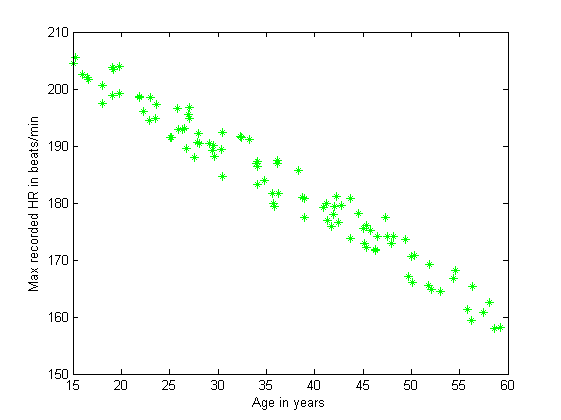
\includegraphics[width=\textwidth]{age_hr_scatter.png}
		\caption{A scatter plot of max HR against age}
		\label{fig:agehr_scatter}
	\end{center}
\end{figure}
Consult the help documentation for the \textbf{regress} function for information on how to use the function.  
We will make use of a constant term so need to add a column of ones to our age data (X).
We can use the \textbf{ones} function to create a column, with as many rows as the matrix: \textbf{D}.

Create the X values from the ages and then use the \textbf{regress} function to create the regression model and extract the statistical data.
\begin{lstlisting}[style=Matlab-editor]
>> age = [ones(size(D(:,1))) D(:,1)];
>> hr = D(:,2);
>> [m,~,~,~,stats] = regress(hr, age);
\end{lstlisting}
Side note: notice the use of \textbf{size} as input to \textbf{ones}; this is a common and important tactic when scripting an analysis.
Look at the output of the \textbf{size} function, as used above:
\begin{lstlisting}[style=Matlab-editor]
size(D(:,1)) % size of column 1

ans = 

   100     1
\end{lstlisting}
We could have entered \textbf{100} and \textbf{1} as input to \textbf{ones} to get a 100 x 1 column vector of ones; however, using the size of a variable in your workspace allows flexibility.
For example, imagine you wanted to add the data for one more participant, making your column vector grow to 101 x 1.
Had you \emph{hard-coded} the \textbf{100} and \textbf{1} as input, you would have to change every line of code that relied on there being 100 rows, using \textbf{size} requires no changes: it would now output 101 and 1.
Back to the module...

The variable \textbf{m} has two elements.  Since this is a linear regression these values correspond to the constants, $m_{0}$ and $m_{1}$, in the standard equation of a line:
\begin{equation*}
Y = m_{0} + m_{1}X
\end{equation*}
where\\
\begin{equation*}
m_{0} = 219.744
\end{equation*}
and\\
\begin{equation*}
m_{1} = -0.9997
\end{equation*}
It is clear that our result is very close to the estimation that:
\begin{equation*}
Y = 220 - X
\end{equation*}
The \textbf{stats} variable has the $R$-square and $F$ statistic, the $p$-value for the full model, and an estimate of the error variance.  
Add the regression line to the plot for ages 0 to 70 years and then add the model and the $R$-square value as a text label.
\begin{lstlisting}[style=Matlab-editor]
% 'hold' axes to add plots without creating new figure
>> hold on 
>> plot((0:70), (b(1) + b(2)*(0:70)));
>> text(20, 210, 'y = 219.744 - 0.9997x (R^ 2 = 0.9596)');
\end{lstlisting}
\begin{figure}[H]
	\begin{center}
		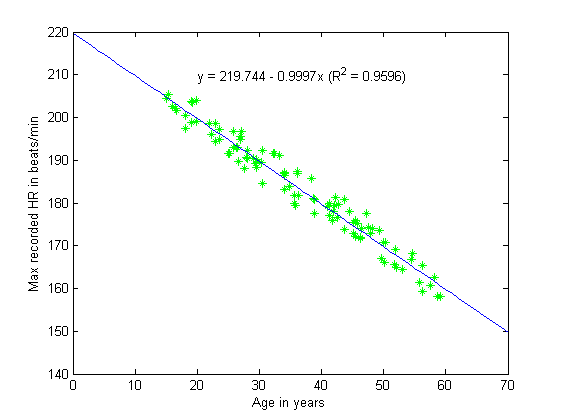
\includegraphics[width=\textwidth]{age_hr_regress.png}
		\caption{A linear regression of HR against Age}
		\label{fig:agehr_regress}
	\end{center}
\end{figure}
Again, whenever you see a new function used, get in the habit of looking up its help documentation, e.g.~ ">> doc text".
The \textbf{text} function allows us to add text to the plotting area. 

\section{$t$-tests}
Import the data from the file \textbf{`ttest.csv'} into the workspace.  
Begin reading at line 2 to skip the header.  
This file contains pre and post-intervention data across various measures for 32 participants.  
The results are from a fictitious long-term fitness intervention study.

\subsection{One-sample and paired-sample \emph{t}-test}
MATLAB's \textbf{ttest} function can be used to perform a one-sample or paired-sample \emph{t}-test.  
We will begin by calculating the change in weight throughout the study.  
This will give us a change score (one sample) for each participant.  
We can take the mean value of this result to see the average amount and direction of weight change.
\begin{lstlisting}[style=Matlab-editor]
>> tdata = csvread('data/ttest.csv', 1)
>> chgWeight = tdata(:,4)-tdata(:,3);
>> mean(chgWeight)

ans =

   -4.9125
\end{lstlisting}
We can now use these change scores to perform a \emph{t}-test of the null hypothesis that the changes are a random sample from a normal distribution with a given mean, \textbf{m}, and unknown variance, against the alternative that the mean is not \textbf{m}.  
We will return to the hypothesis outcome, \textbf{h} (where $h = 1$ indicates a rejection of the null hypothesis and $h = 0$ indicates a failure to reject the null hypothesis) and the $p$-value of the test.  
We will use the default values of mean, \textbf{m}, as 0 (no weight change), an alpha value of 0.05 and a two-tailed test.
\begin{lstlisting}[style=Matlab-editor]
>> [h, p] = ttest(chgWeight,0);
\end{lstlisting}
The result shows that the null-hypothesis was rejected, $h = 1$, since the $p$ value ($p$ = 0.0377) is less than the 0.05 threshold.  
Confirm that reducing the significance level to an alpha value of 0.01, 1\%, would result in a failure to reject the null hypothesis.
\begin{lstlisting}[style=Matlab-editor]
>> h = ttest(chgWeight, 0, 0.01)

h = 

   0
\end{lstlisting}
In the previous example we used single samples that were created as a change score pre and post intervention.  
It then follows that the null hypothesis would be that the mean was 0.  
We could have taken the raw values and used a paired-sample \emph{t}-test to perform a similar statistical analysis.  
Verify that the result would, as expected, produce an identical outcome:
\begin{lstlisting}[style=Matlab-editor]
>> [h, p] = ttest(tdata(:,4), tdata(:,3));
\end{lstlisting}
We will now use the gender information, in column 2, to investigate the effect the intervention had on pre/post BMI scores within each sex.  
Extract the indices of males and females and perform a paired-sample \emph{t}-test on each group.
\begin{lstlisting}[style=Matlab-editor]
>> males = tdata(:,2) == 1;
>> females = tdata(:,2) == 2;	
>> [hF, pF] = ttest(tdata(females,5), tdata(females,6));
>> [hM, pM] = ttest(tdata(males,5), tdata(males,6));
\end{lstlisting}
Verify that effect is significant in one gender group but not in the other.  

\subsection{Two-sample \emph{t}-test}
We will now perform an unpaired two-sample, or \emph{`independent samples'} \emph{t}-test on the same body weight data as before.
\begin{lstlisting}[style=Matlab-editor]		
>> [h2, p2] = ttest2(tdata(:,4),tdata(:,3));
\end{lstlisting}
Compare this result to the paired-sample results from before (\textbf{h} and \textbf{p}), notice the difference.  
In this second case we are using the same set of data, but we are not treating the observations (rows) as paired, just as two separate samples.  
This type of test does not have the same level of power as a paired sample test and this shows in the change of the result.  
This highlights the importance of choosing the correct statistical model as you can get a very different result, even when using exactly the same data!

\section{Analysis of Variance}
\subsection{One-way analysis of variance}
Using the same data set as before we will look at running an analysis of variance, or ANOVA, on the weight change scores by gender.  
First we need to create a grouping variable.  
We could simply use the gender column in the data matrix but this would not give much information on the resulting output.  
Instead we will create a variable that has the strings "'Male'" or "'Female'" relating to each value in the gender column, where 1 = `Male' and 2 = `Female'.  
Once this variable has been created we will use MATLAB's \textbf{anova1} function to perform a one-way analysis of variance.
\begin{lstlisting}[style=Matlab-editor]
>> gender = cell(size(tdata(:,2))); % cell array
>> gender(tdata(:,2) == 1) = {'Male'};		
>> gender(tdata(:,2) == 2) = {'Female'};		
>> [p... stats] = anova1(chgWeight, gender)

p =
   
   0.0098
   
>> [] multcompare(stats);
   
>> [gnames(c(:,1)), gnames(c(:,2)), num2cell(c(:,3:6))]

ans =

   1x6 cell array
	
   {'Male'}    {'Female'}    {[-19.8815]}    {[-11.4254]}    {[-2.9693]}    {[0.0098]}
	
\end{lstlisting}
% not actually necessary to make the cell, could do p = anova1(chgWeight, tdata(:,2)), but the factor levels wouldn't be labelled.
The following figures should be displayed to show the results of the analysis.
\begin{figure}[H]
	\begin{center}
		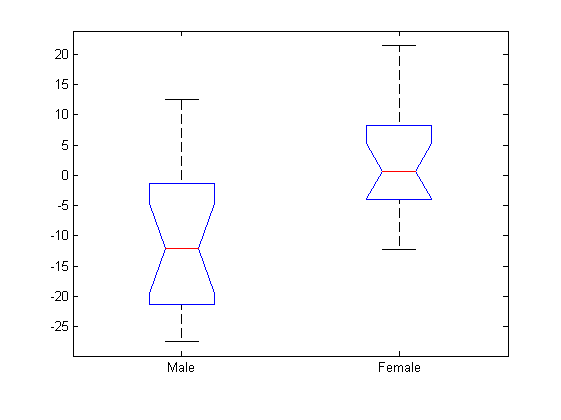
\includegraphics[width=\textwidth]{anova_boxplot.png}
		\caption{A box plot showing the change in weight for males and females}
		\label{fig:anova_boxplot}
	\end{center}
\end{figure}
\begin{figure}[H]
	\begin{center}
		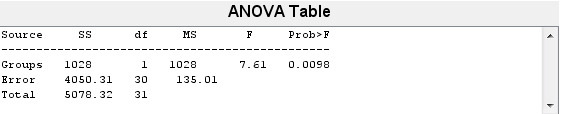
\includegraphics[width=\textwidth]{anova_table.png}
		\caption{The table output from the ANOVA function}
		\label{fig:anova_table}
	\end{center}
\end{figure}
From the table and from the output variable, \textbf{p}, we can see that we should reject the null hypothesis that the two groups are drawn from a population with the same mean.  
This result indicates that there is a significant difference ($p = 0.0098$) in the average weight change between men and women during the intervention.
We could also say that, if the samples were drawn from the same population we would only expect differences of this magnitude about 1\% of the time in repeated experiments.
Additionally, the box plot clearly shows how these changes in men and women differ.

In summary we can infer the following from the ANOVA and previous $t$-tests:

\begin{itemize}
	\item There was a significant loss in body weight in the overall sample group, $t(31) = -2.17$, $p = .038$, 95\% CI $[-9.53, -0.30]$.
	\item However, the ANOVA indicated that there was a significant difference in the nature of the change between the two gender groups $F(1,30) = 7.61$, $p = .010 $, 95\% CI [-19.89, -2.97].
	\item The \emph{t}-tests within the gender groups showed that there was a highly significant loss in body weight in the male participants $t(17) = 2.22$, $p = 0.040$, 95\% CI $[0.30, 11.44]$, and only a slight non-significant increase in body weight for females $t(13) = 0.72$, $p = .483$, 95\% CI $[-4.06, 8.13]$.
\end{itemize}

\subsection{Two-way analysis of variance}
In this section we will introduce the two-way ANOVA for comparing the means across a combination of two factors.  
We will do this by using one of MATLAB's examples found in the Help documentation.  
Load the help documentation for using MATLAB's two-way ANOVA function, called \textbf{anova2}, i.e.~ ">> doc anova2".
This documentation has a detailed explanation of all of the possible ways in which the function can be used.  
Read this information and then follow the example shown.  
This example will make use of one of the internal MATLAB dataset called \textbf{popcorn}.

\subsubsection{Further statistical analysis}
At this point, you may decide to export your data to a file format of your choice and conduct your statistical analysis using other software such as R or SPSS.
MATLAB's statistical toolbox is intended mainly for engineering purposes and lacks some of the tests and conventions necessary for sports and health science.

\end{document}

%This time we will perform another two-way ANOVA and use two grouping variables to set up the analysis.  
%Use the \textbf{tdfread} function to load in some data from the file called \textbf{`anova.csv'}.  
%Set the delimiter character to a comma, `,'.  
%This file contains data from a study involving a maximal duration running protocol.  
%Each participant completed the run under two conditions, when hydrated with a sports drink and also when hydrated with water alone.  
%Participants were separated into two groups, those that had trained and competed exclusively or almost exclusively using sports drinks for many years and those that had never or very rarely used sports drinks.
%\begin{lstlisting}[style=Matlab-editor]
%>> tdfread('anova.csv', ',');
%\end{lstlisting}
%Three variables, \textbf{Condition}, \textbf{Duration} and \textbf{Group}, should have been loaded into the workspace.  
%The \textbf{Duration} variable has the amount of time, in minutes, that a runner could maintain running a fixed pace of 15 km/h on a treadmill.  
%The other two variables contain the grouping information.
%
%Let us assume that our hypothesis in this study is that the change in performance due to hydrating with sports drink instead of water will be different depending on whether an athlete has had a significant exposure to the sports drink beforehand.  
%This will show as an interaction between \textbf{Group} and \textbf{Condition} in the two-way ANOVA.







